% Options for packages loaded elsewhere
\PassOptionsToPackage{unicode}{hyperref}
\PassOptionsToPackage{hyphens}{url}
%
\documentclass[
]{article}
\usepackage{lmodern}
\usepackage{amssymb,amsmath}
\usepackage{ifxetex,ifluatex}
\ifnum 0\ifxetex 1\fi\ifluatex 1\fi=0 % if pdftex
  \usepackage[T1]{fontenc}
  \usepackage[utf8]{inputenc}
  \usepackage{textcomp} % provide euro and other symbols
\else % if luatex or xetex
  \usepackage{unicode-math}
  \defaultfontfeatures{Scale=MatchLowercase}
  \defaultfontfeatures[\rmfamily]{Ligatures=TeX,Scale=1}
\fi
% Use upquote if available, for straight quotes in verbatim environments
\IfFileExists{upquote.sty}{\usepackage{upquote}}{}
\IfFileExists{microtype.sty}{% use microtype if available
  \usepackage[]{microtype}
  \UseMicrotypeSet[protrusion]{basicmath} % disable protrusion for tt fonts
}{}
\makeatletter
\@ifundefined{KOMAClassName}{% if non-KOMA class
  \IfFileExists{parskip.sty}{%
    \usepackage{parskip}
  }{% else
    \setlength{\parindent}{0pt}
    \setlength{\parskip}{6pt plus 2pt minus 1pt}}
}{% if KOMA class
  \KOMAoptions{parskip=half}}
\makeatother
\usepackage{xcolor}
\IfFileExists{xurl.sty}{\usepackage{xurl}}{} % add URL line breaks if available
\IfFileExists{bookmark.sty}{\usepackage{bookmark}}{\usepackage{hyperref}}
\hypersetup{
  hidelinks,
  pdfcreator={LaTeX via pandoc}}
\urlstyle{same} % disable monospaced font for URLs
\usepackage{graphicx}
\makeatletter
\def\maxwidth{\ifdim\Gin@nat@width>\linewidth\linewidth\else\Gin@nat@width\fi}
\def\maxheight{\ifdim\Gin@nat@height>\textheight\textheight\else\Gin@nat@height\fi}
\makeatother
% Scale images if necessary, so that they will not overflow the page
% margins by default, and it is still possible to overwrite the defaults
% using explicit options in \includegraphics[width, height, ...]{}
\setkeys{Gin}{width=\maxwidth,height=\maxheight,keepaspectratio}
% Set default figure placement to htbp
\makeatletter
\def\fps@figure{htbp}
\makeatother
\setlength{\emergencystretch}{3em} % prevent overfull lines
\providecommand{\tightlist}{%
  \setlength{\itemsep}{0pt}\setlength{\parskip}{0pt}}
\setcounter{secnumdepth}{-\maxdimen} % remove section numbering
\ifluatex
  \usepackage{selnolig}  % disable illegal ligatures
\fi
\newlength{\cslhangindent}
\setlength{\cslhangindent}{1.5em}
\newenvironment{cslreferences}%
  {\setlength{\parindent}{0pt}%
  \everypar{\setlength{\hangindent}{\cslhangindent}}\ignorespaces}%
  {\par}

\author{}
\date{}

\begin{document}

\newcommand{\matr}[1]\textbf

\{\#1\}

\newcommand{\vect}[1]{\vec{#1}}

\hypertarget{to-my-dear-supervisors}{%
\section{To my dear supervisors}\label{to-my-dear-supervisors}}

Dear Professor Likos! Dear Dr.~Bianchi!

Professor Likos, I hope you're enjoying your vacation.

You haven't heard from me in a while because I was on vaction too, but I
have started my work on the thesis. I will review what we discussed in
person and online with Dr.~Bianchi, and I hope you are as interested in
the research question as I am. Dr.~Bianchi, if you have suggestions for
adapting dimensions/parameters of the situation (fluid flow through 2d
cross section of pipe with cylindrical obstacles) or even tweak the
situation, I would love to hear your suggestions too. I hope I depicted
the situation somewhat well below. I thought it would be interesting to
not only try obstacles that are regularly spaced, all the same size, but
try a more heterogeneous situation. But that is still a little ways down
the road, so I'll have to see about that.

Progress-wise I'd say I'm still at the beginning. All the work here has
been done in about 1 week. I'm working on the collision step now. It
took a lot of time to get familiar with C++ again, and to find out how
best to test my results. I think I have found a good way to do this,
called unit testing, which basically means you test every unit of your
program separately and make sure they work under various circumstances,
to make debugging easier later down the road and also to add more
credibility to my results.

Please do not worry if the writing style is sometimes informal, and at
other times formal. I meant it to be that way, as some sections are
unfinished/jumbled down thoughts/still expanding/experimenting. Also,
the citing style is not the final version either, unfortunately, I
cannot change it at the moment.

I'd be happy to hear your guidance and if everything is looking good, or
if you suggest I focus more on other areas. If you have a lot to tell me
I'd be happy to meet over Zoom/Teams or in person.

Where possible, I've not cited Wikipedia, or added other sources. Is it
still okay if I cite Wikipedia, or is that completely undesirable?

All the best,

Chris

\hypertarget{mpcd-simulation-of-polymers-in-solution}{%
\section{MPCD simulation of polymers in
solution}\label{mpcd-simulation-of-polymers-in-solution}}

This notebook will serve as the documentation of our efforts and results
for my Bachelor's Thesis. The goal of this thesis will be the study of
short/long-chained polymers in a liquid thats flowing around obstacles.
The liquid will be simulated with MPCD, or ``Multi Particle Collision
Dynamics''.

I chose the language C++ for its familiar object-oriented nature and its
proven execution-time. Output of the simulation will mostly be analysed
in Python, specifically with Jupyter Notebook for a blend of beautiful
visualizations and convenience. For simplification, the situation will
be studied in 2D. The situation we specifically discussed is shown
below.

\begin{figure}
\centering
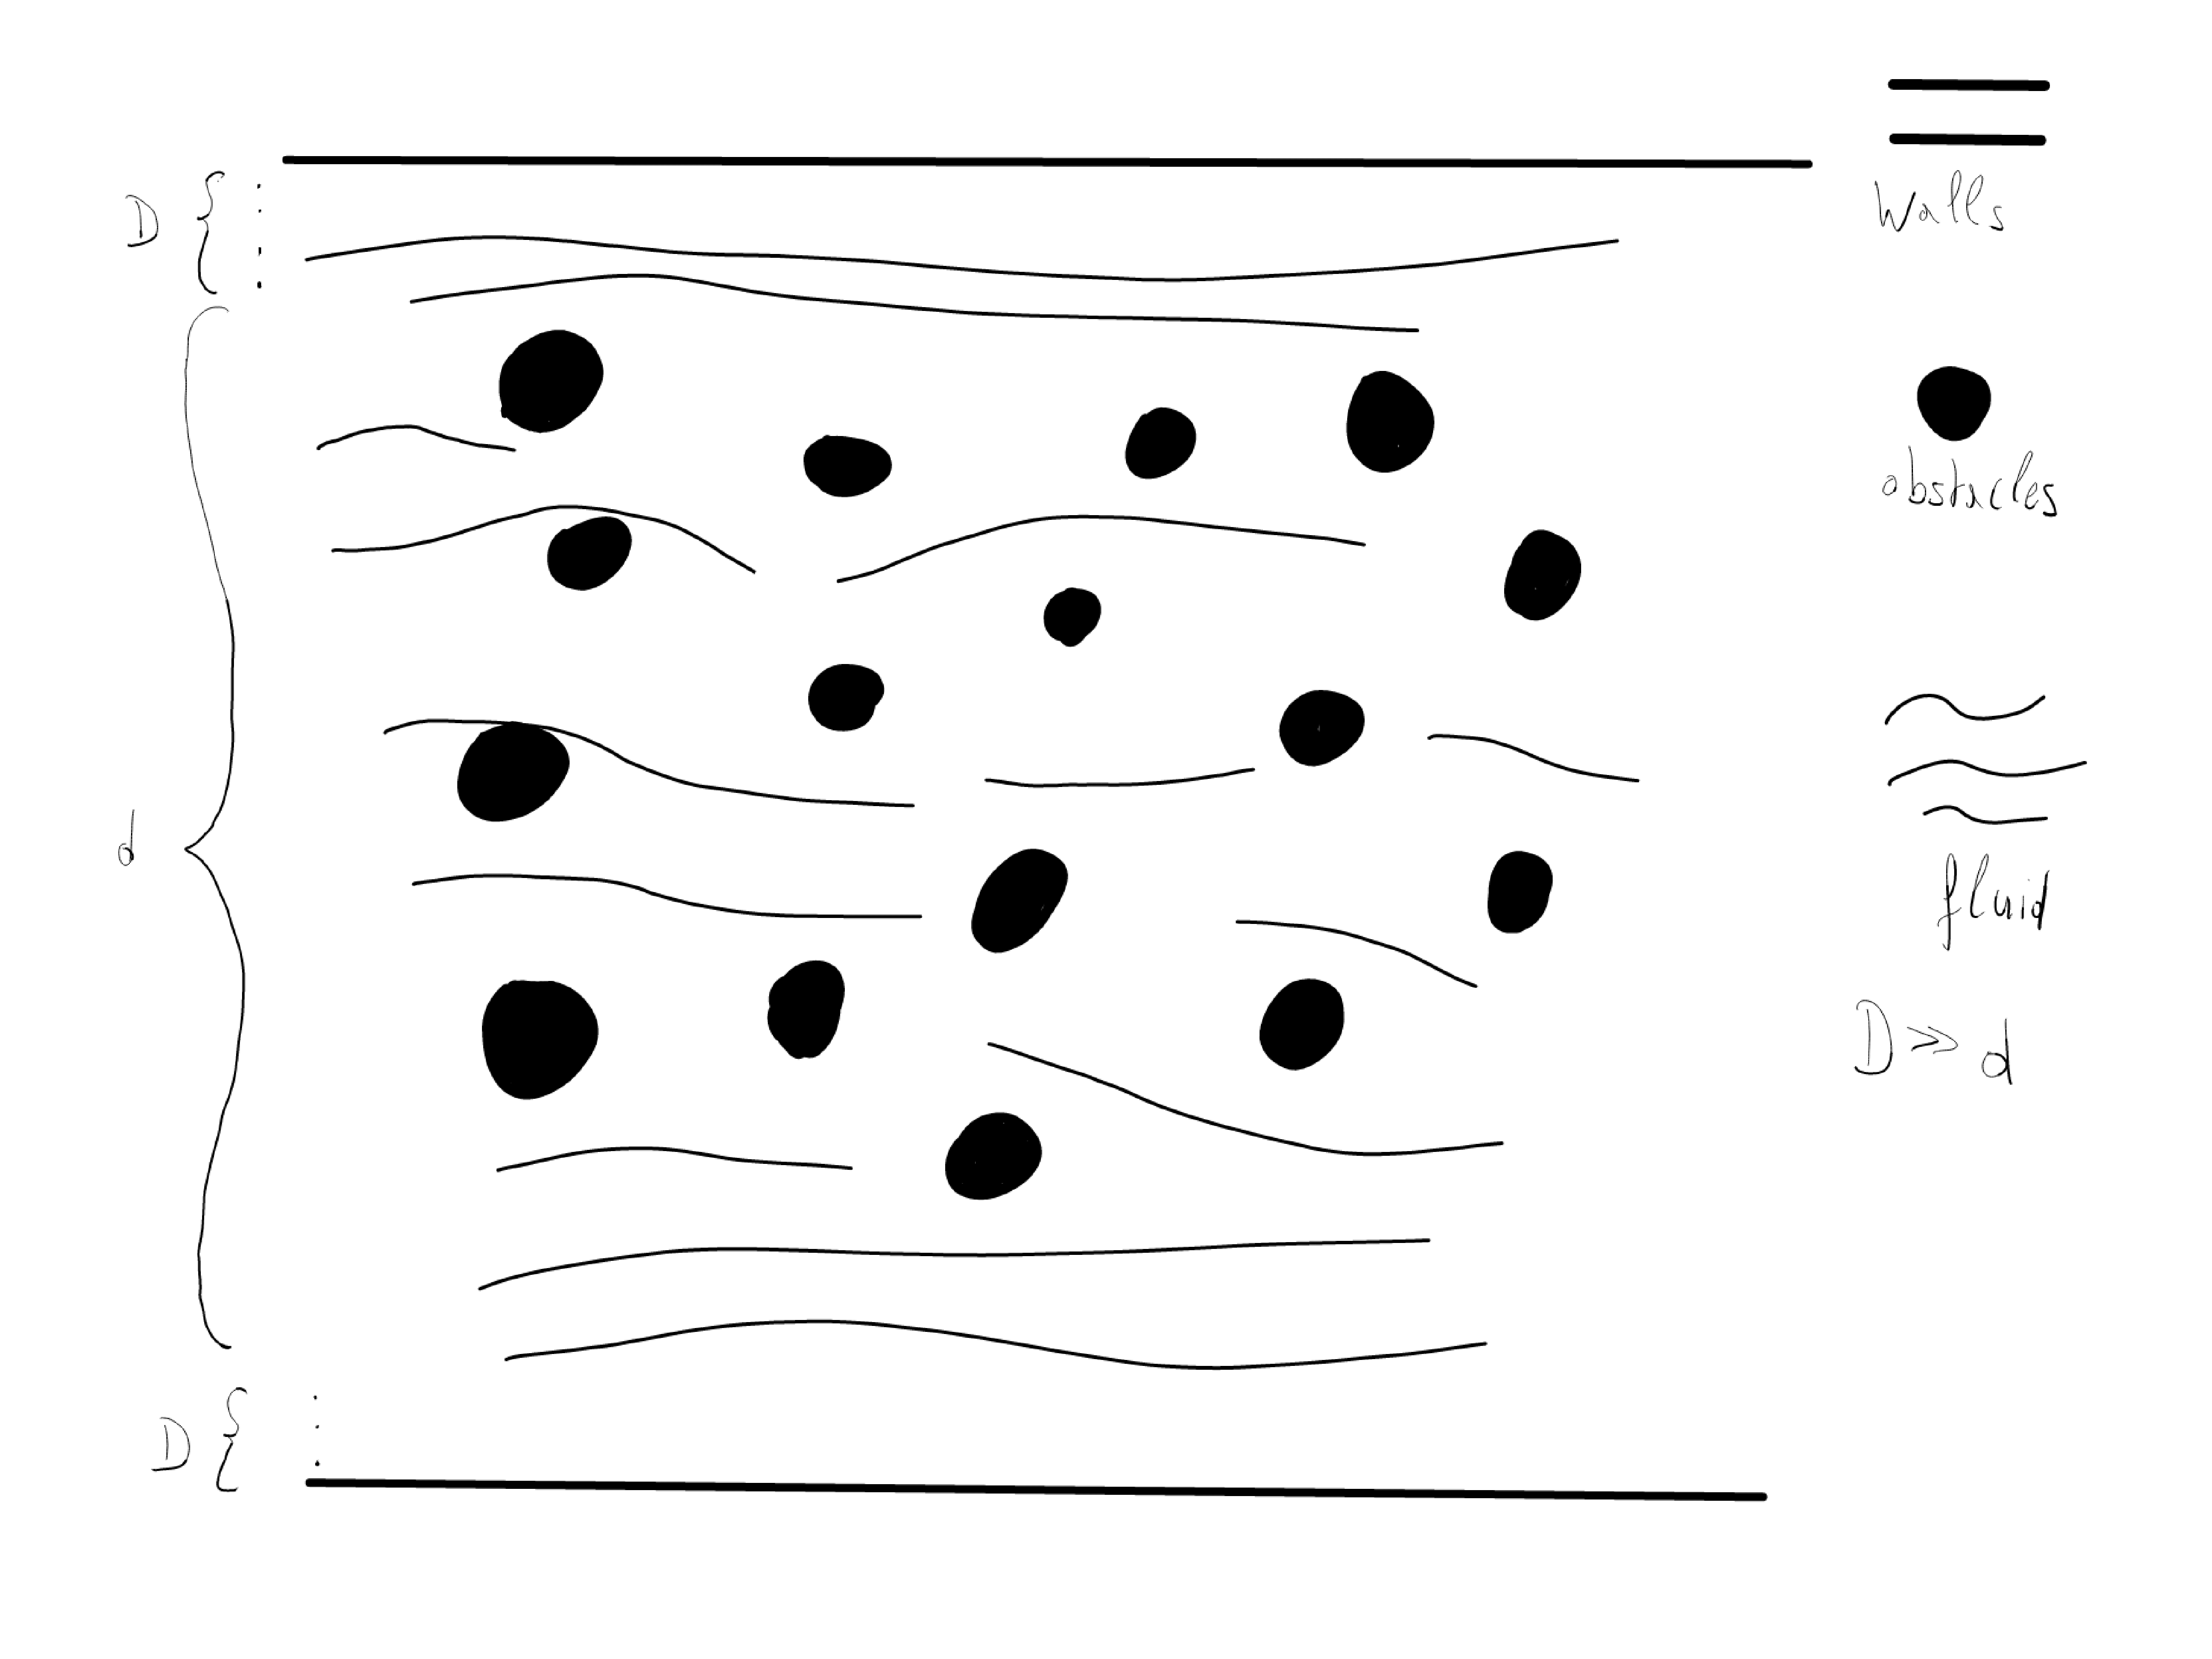
\includegraphics{Assets/MPCD_Situation.png}
\caption{Situation}
\end{figure}

\hypertarget{open-questions-description-of-situation}{%
\subsubsection{Open questions \& Description of
situation}\label{open-questions-description-of-situation}}

For these questions, I need to expand the program to even consider them.
If I get close and still have no idea how to go about them, I will
contact Maximilian Liebetreu (I think he was there when we first met,
I'm sorry I can't remember exactly). Are there other people I can
contact for the programming/implementation details?

The fluid flows from the -x direction through the 2D cross-section of
some vessel. In this vessel there are cylindrically shaped objects,
through which the fluid cannot pass. (-\textgreater How will I simulate
the obstacles, are they solid non-deformable, are they soft \& elastic,
..?) (-\textgreater{} Methods: create a lot of particles and immobilize
them?, check for collision between particles and obstacles on a per
particle basis? (this will probably be too expensive computationally))

What happens when fluid goes out of bounds? (-\textgreater Should
particles that go too far in the +x direction be destroyed and new ones
created from the -x direction, simulating continuous flow?)

Finally, polymers will be introduced into the fluid and their behavior
studied. We might imagine this ``vessel'' as a blood vessel and the
obstacles as cells moving around in the bloodstream, for example.
(-\textgreater{} For the polymers, you told me I should wait until the
MPCD is really working)

\hypertarget{introduction}{%
\section{Introduction}\label{introduction}}

Multiparticle collision dynamics (MPCD), also known as Stochastic
Rotation Dynamics (SRD)(Gompper et al., 2009) is a technique originally
introduced to study the dynamics of complex fluids such as polymers in
solution. Besides MPCD, there exist other mesoscopic models that have
been constructed for this purpose, such as Langevin, Direct Simulation
Monte Carlo and lattice Boltzmann methods.(Malevanets \& Kapral, 1999)
We only concern ourselves with the application of MPCD, it follows that
any comparison between methods are out of the scope of this thesis.

The MPCD technique models the fluid using particles, their positions and
velocities are treated as continuous variables. The system is divided up
into cells that have no restriction on the number of particles, each of
the cells is part of a regular lattice. The dynamics is split into two
parts: Particle streaming and multiparticle collision dynamics. Particle
streaming is treated exactly for each particle in the system, while the
collision step is approximated on a cell level. The multiparticle
collision dynamics conserves mass, momentum and energy and leads to the
correct hydrodynamical equations.(Malevanets \& Kapral, 1999) The
streaming and collision step are described in more detail in (TODO).

\hypertarget{how-does-mpcd-work}{%
\section{How does MPCD work?}\label{how-does-mpcd-work}}

The system we are modelling consists of \(N\) particles with mass \(m\),
position \(\vec{r_{i}}\) and velocity \(\vec{v_{i}}\), where
\(i \in \{1, 2, \dots, N\}\). One timestep shall correspond to having
calculated all the new particle positions and velocities in the
streaming and collision steps, respectively. For each of the N
particles, the streaming and collision steps are applied, and this
pattern is repeated until the wanted number of timesteps have elapsed.

\hypertarget{the-streaming-step}{%
\subsection{The streaming step}\label{the-streaming-step}}

The streaming step is very straightforward. The particle positions are
simply updated according to

\begin{equation}
\vec{r_{i}} \rightarrow \vec{r_{i}} + \Delta t \cdot \vec{v_{i}}\textrm{,}
\end{equation}

where \(\Delta t\) is a small time interval.(Gompper et al.,
2009)(Malevanets \& Kapral, 1999)

\hypertarget{the-collision-step}{%
\subsection{The collision step}\label{the-collision-step}}

The collision step is somewhat more complicated. It involves the mean
velocity of all particles in a particular cell, \(\vec{V_c}\), the
velocity of the particle \(i\) \(\vec{v_i}\) and a rotation matrix
\(\textbf(\alpha)\). The vector \(\vec{v_i}\) is rotated relative to the
mean velocity \(\vec{V_c}\) of all particles in cell \(c\), cell \(c\)
being the cell which particle \(i\) belongs to. It is shown in
(Malevanets \& Kapral, 1999) that the rule,

\begin{equation}
\vec{v_i} \rightarrow \vec{V_c} + \textbf(\alpha) [\vec{v_i} - \vec{V_c}] \textrm{,}
\end{equation}

conserves mass, momentum and energy. The rotation matrix
\(\textbf(\alpha)\) is a simple 2d rotation matrix

\begin{equation}
R(\alpha) = 
\left[ \begin{array}{rr}
cos(\alpha) & -sin(\alpha) \\
sin(\alpha) & cos(\alpha) \\
\end{array}\right]
\end{equation}

It is the same for all particles of a cell, but since \(\alpha\) is
sampled randomly, will probably differ from cell to cell. The mean
velocity of a cell is defined as

\begin{equation}
\vec{V_c} = \frac{1}{N_c} \sum_{i=1}^{N_c} \vec{v_i} \textrm{,}
\end{equation}

where \(N_c\) is the number of particles in the cell.(Malevanets \&
Kapral, 1999)

\hypertarget{pseudo-random-number-generation}{%
\section{(Pseudo) Random Number
Generation}\label{pseudo-random-number-generation}}

One of the pillars of this thesis is the generation of random rotation
angles for the rotation matrix needed in the collision step. This proved
to be somewhat difficult. First, the standard algorithm of the C++
standard library was tried, but it didn't qualify because it performed
poorly in comparison to the second and third algorithms tried, which are
called ``Mersenne Twister'' and ``xoshiro256++'',
respectively.(Wikipedia contributors, 2020c)(cppreference contributors,
2020)(Vigna, Sebastiano, 2020)

The Mersenne Twister was implemented using the C++ standard library. The
xoshiro256++ was implemented using Sebastian Vigna's code with some
additions.(Vigna, Sebastiano, 2020)

To compare algorithms, and also to make sure that the implementation of
the xoshiro256++ is right, a \(\chi^2\) test for discrete observations
was used. The generated angles in the interval \([0, 2\pi)\) were split
into \(k+1\) buckets, where \(k\) is the number of degrees of freedom of
the \(\chi^2\) distribution. The test error

\begin{equation}
T = \sum_{b=1}^{k+1}{\frac{(N_o - E[N_b])^2}{E[N_b]}},
\end{equation}

where \(E[N_b] = \frac{N}{b}, b \in \{1, 2, \dots , k+1\}\) is the
expected bucket size, is compared to \(\chi^2_{1-\alpha, k}\), where
\(\alpha\) is the signifigance level. The null hypothesis

\[
H_0: \textrm{The angles are distributed uniformly in the interval } [0, 2 \pi)
\]

is tested against the alternative hypothesis

\[
H_1: \textrm{The angles are not distributed uniformly in the interval } [0, 2 \pi) \textrm{.}
\]

If the test should have significance level \(\alpha\), \(H_0\) is
rejected if \(T \ge \chi^2_{1-\alpha, k}\).(Frühwirth, Rudolf,
n.d.)(Wikipedia contributors, 2020a)(Wikipedia contributors, 2020b)

The results of the \(\chi^2\) test are summarised in {[}TODO: Table, and
table formatting{]}.

\begin{table}[]
\begin{tabular}{|l|c|r|r|}
\textbf{k} & \textbf{chisquared[TODO]} &\textbf{observed MT} & \textbf{observed xoshiro} \\
1                              & 3.841           & 4.709                                    & 0.551                                         \\
2                              & 5.991            & 6.211                                    & 0.58                                          \\
3                              & 7.815                          & 8.137                                    & 1.263                                         \\
4                              & 9.488                          & 11.506                       & 1.776                                         \\
5                              & 11.070                          & 10.954                                   & 3.783                                         \\
6                              & 12.592                          & 19.849                                   & 4.565                                         \\ 
7                              & 14.067                          & 12.545                                   & 3.339                                         \\
8                              & 15.507                          & 14.802                                   & 4.946                             \\
9                              & 16.919                           & 14.101                       & 3.196                                         \\
10                             & 18.307                          & 15.701                       & 5.794                                         \\ 
11                             & 19.675                          & 19.148                                   & 9.452                                         \\
12                             & 21.026                         & 17.072                                   & 6.947                                         \\ 
13                             & 22.362              & 20.366                                   & 10.734                            \\
14                             & 23.685                          & 18.033                                   & 6.426                                         \\ 
15                             & 24.996              & 15.477                                   & 6.75                                          \\
16                             & 26.296                          & 18.604                                   & 8.554                                         \\
17                             & 27.587                           & 21.79                                    & 13.028                            \\
18                             & 28.869                         & 26.316                                   & 9.882                                         \\ 
19                             & 30.144             & 26.845                                   & 14.323                                       
\end{tabular}
\end{table}

As we can see, both generators pass the \(\chi^2\) test and we do not
have to reject our null hypothesis \(H_0\).

Visually, we can examine the generated buckets of both random generators
in {[}TODO{]} the following plot.

\begin{figure}
\centering
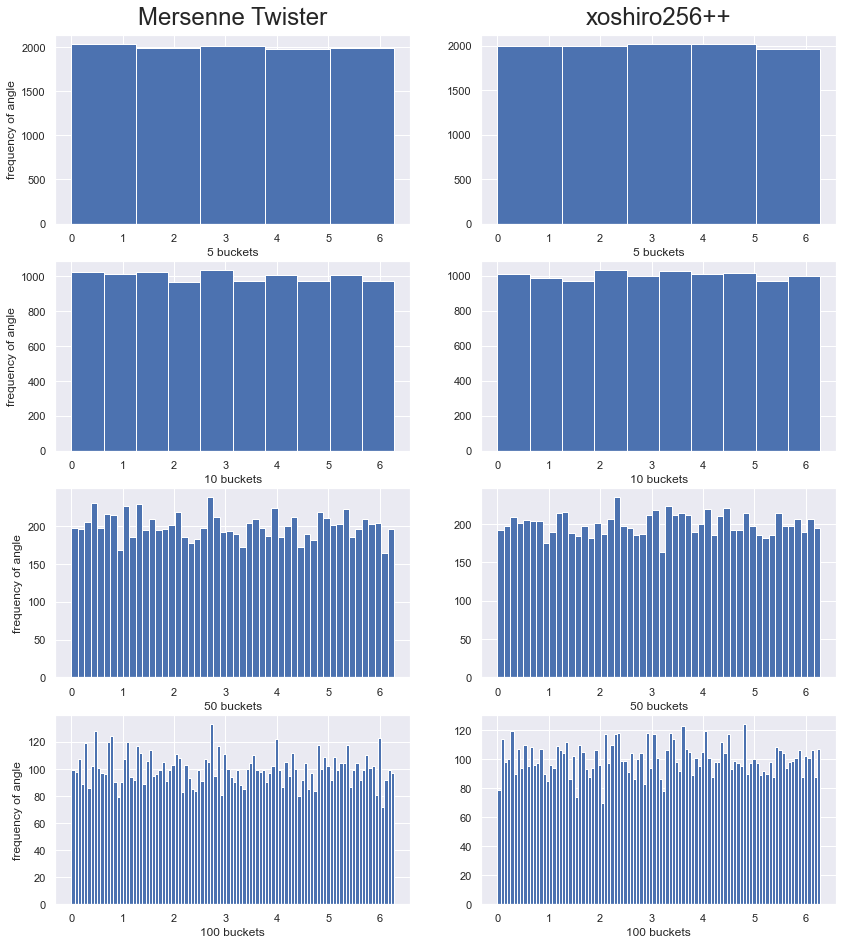
\includegraphics{thesis_files/thesis_24_0.png}
\caption{png}
\end{figure}

\begin{figure}
\centering
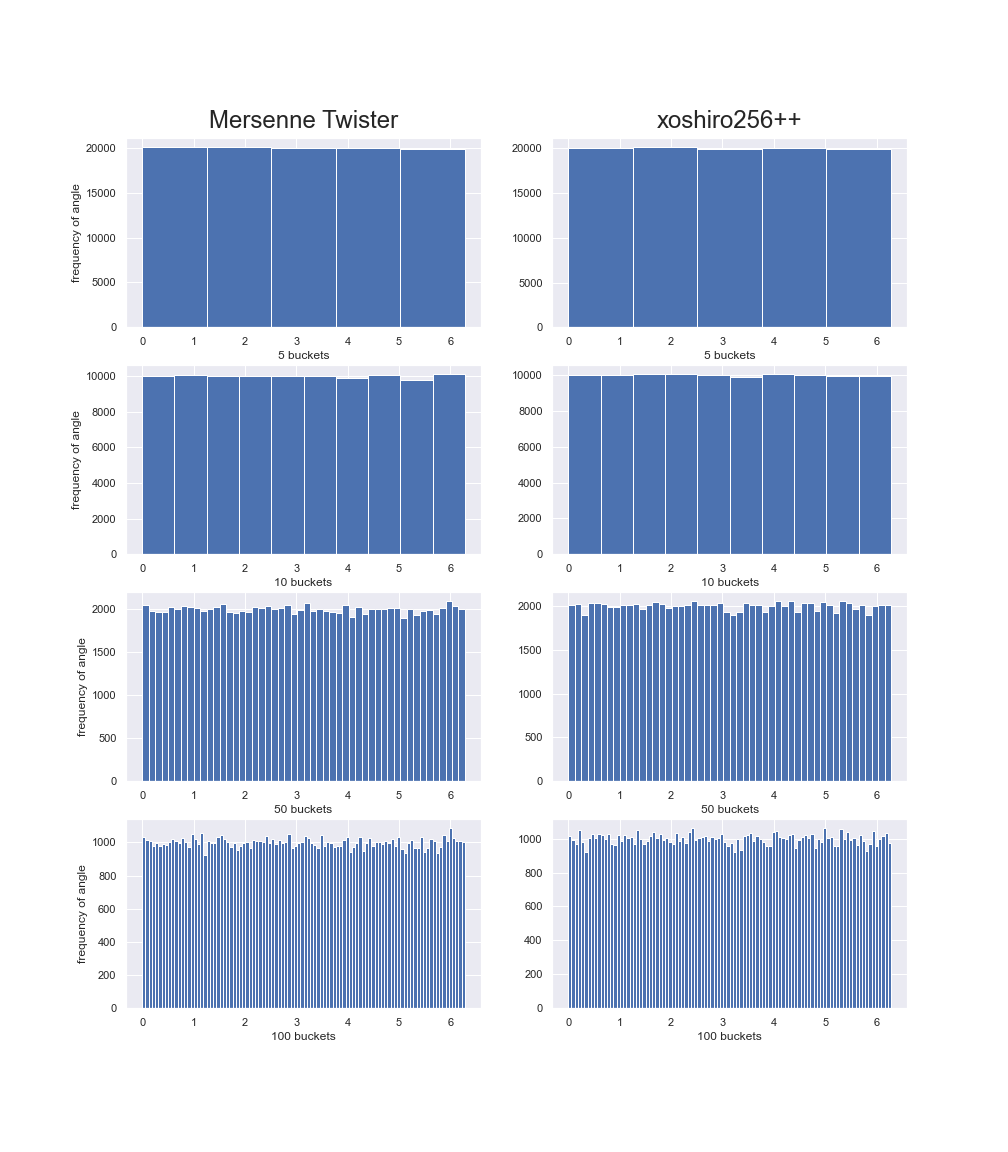
\includegraphics{Assets/angle_buckets.png}
\caption{A histogram of different bucket sizes generated by MT and
xoshiro256++}
\end{figure}

The Mersenne Twister has been known to fail certain statistical tests
since its inception, by virtue of its mathematical characteristics.
There exist other algorithms that are designed to be faster and that do
not fail any known statistical tests.(Vigna, 2019) Ultimately, the
xoshiro256++, developed by Sebastian Vigna and David Blackman, was used.
It is a variant of the xorshift algorithm, which extends the bit-shift
and xor methods by bitrotation, making it still very fast, and more
``random'' than the xorshift.(Wikipedia contributors, 2020e)(Vigna,
Sebastiano, 2020)

Note that testing a (pseudo) random number generator is usually much
more involved than this, but since this has already been done
extensively by other authors, we are satisfied with the \(\chi^2\) test,
simply to test the implementation of the xoshiro256++, since it plays an
important part.(Wikipedia contributors, 2020d)(Vigna, 2019)

\hypertarget{particle-streaming}{%
\section{Particle Streaming}\label{particle-streaming}}

The particle positions were drawn from a uniform real distribution in
the interval \([0, 5)\) for the \(x\)-coordinate, and \([0, 1)\) for the
\(y\)-coordinate. The velocities were initialized to be in the interval
\([-1\% \cdot 5, 1\% \cdot 5)\) for the \(v_x\) component, and
\([-1\% \cdot 1, 1\% \cdot 1)\) for the \(v_y\) component. The results
can be seen {[}TODO{]} below. From the positions in the first row, the
velocities in the second row, particle streaming is applied for 1 and 10
timesteps, respectively.

\begin{figure}
\centering
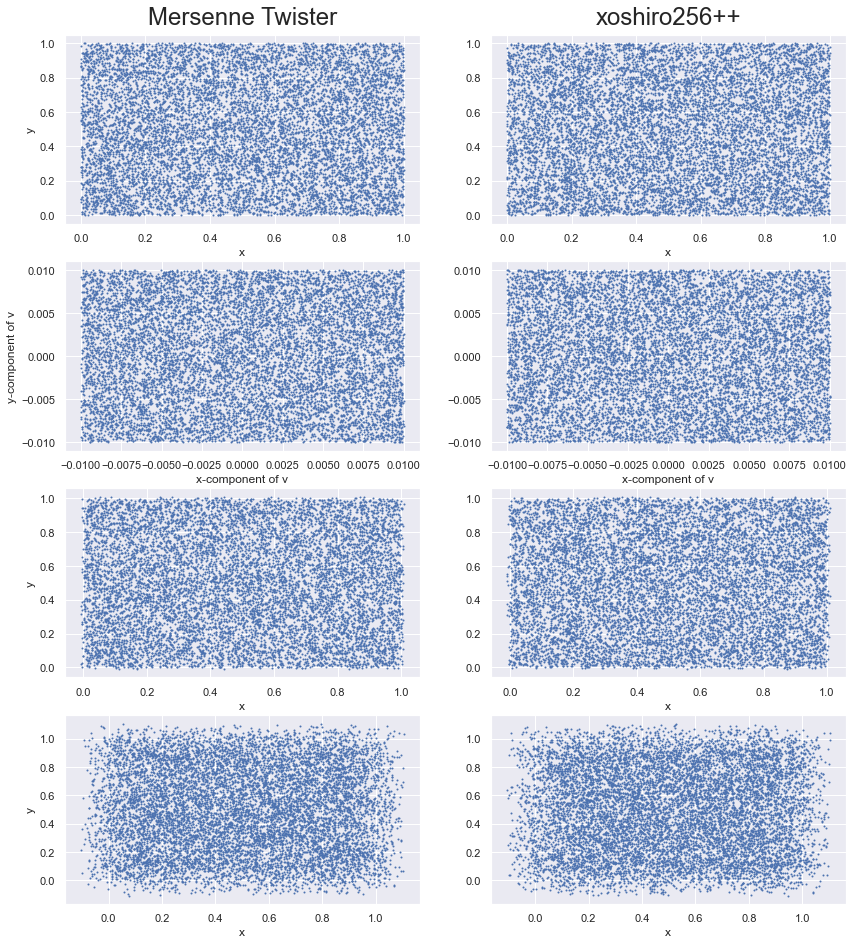
\includegraphics{thesis_files/thesis_29_0.png}
\caption{png}
\end{figure}

\begin{figure}
\centering
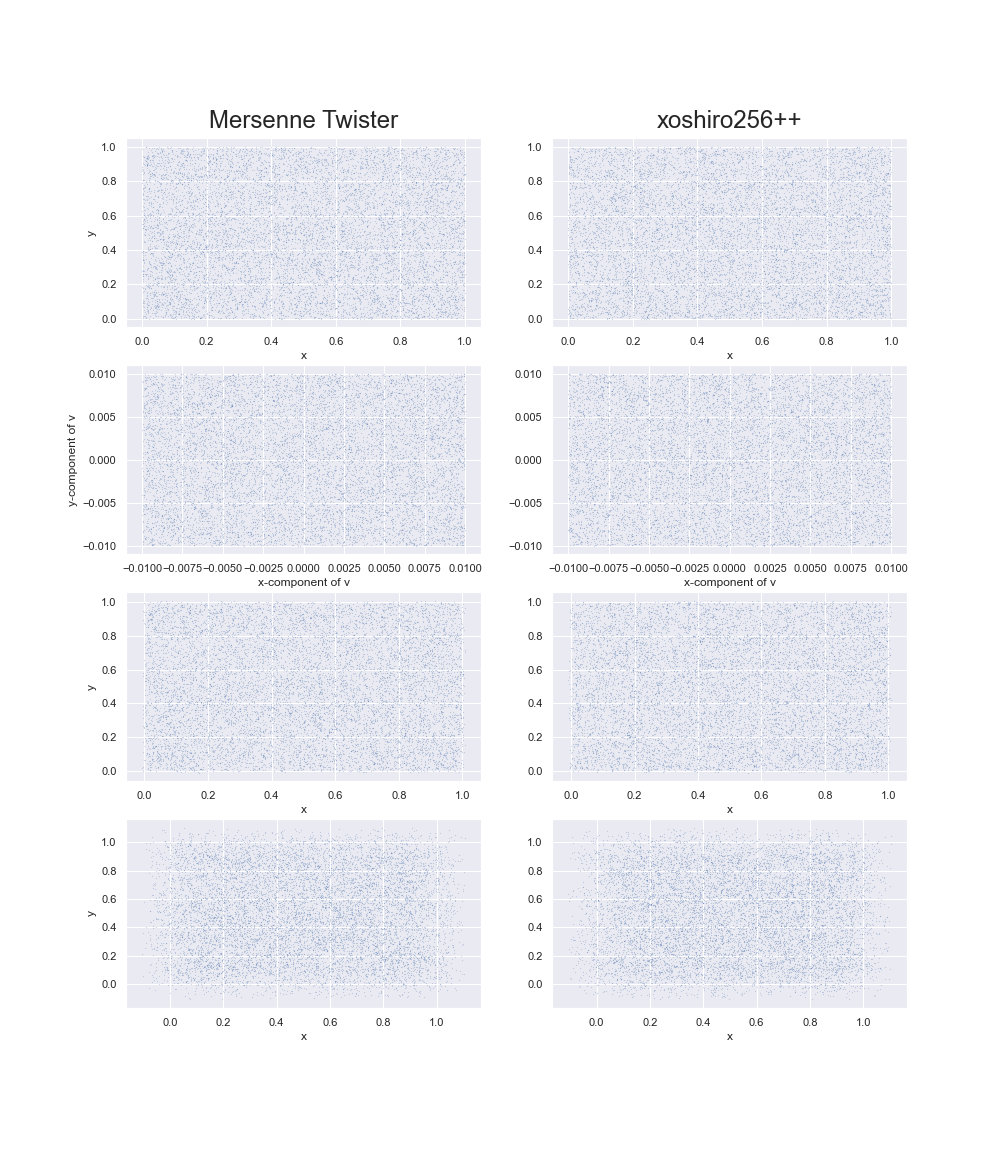
\includegraphics{Assets/particle_streaming.png}
\caption{Particle streaming without collision with MT and with xoshiro}
\end{figure}

We see the x and y coordinates are randomly initialized according to the
shape of the container. Looking closely, one can see that our particles
look very much like noise. The absolute value of the velocity components
are initialized to at most 1\% of their respective dimensions. After one
timestep, some of the particles on the outer ranges have moved out of
bounds, and after ten timesteps, the particles have thinned out
considerably along the edges.

\hypertarget{the-collision-step-1}{%
\section{The collision step}\label{the-collision-step-1}}

\hypertarget{grid}{%
\subsection{Grid}\label{grid}}

Work in progress

\hypertarget{velocity-updating}{%
\subsection{Velocity updating}\label{velocity-updating}}

The velocity of a particle updates according to \begin{equation}
\vec{v_{i}} \rightarrow \vec{V_c} + \textbf(\alpha)[\vec{v_i} - \vec{V_c}],
\end{equation}

where \(\vec{v_{i}}\) is the velocity of the \(i-th\) particle,
\(\vec{V_c}\) is the mean velocity of all particles belonging to cell
\(c\), specified by \(i\)'s position. The matrix

\[
R(\alpha) = 
\left[ \begin{array}{rr}
cos(\alpha) & -sin(\alpha) \\
sin(\alpha) & cos(\alpha) \\
\end{array}\right]
\]

is a simple 2d-rotation matrix. The angle \(\alpha\) is uniformly
sampled from the interval \([0, 2\pi)\) on a per-cell basis.(Malevanets
\& Kapral, 1999)

\hypertarget{refs}{}
\begin{cslreferences}
\leavevmode\hypertarget{ref-cppreference:prng}{}%
cppreference contributors. (2020). \emph{Pseudo-random number generation
- cppreference.com}.
\url{https://en.cppreference.com/w/cpp/numeric/random}

\leavevmode\hypertarget{ref-fruehwirthstat}{}%
Frühwirth, Rudolf. (n.d.). \emph{Wahrscheinlichkeitsrechnung und
Statistik}.

\leavevmode\hypertarget{ref-winkl2009}{}%
Gompper, G., Ihle, T., Kroll, D. M., \& Winkler, R. G. (2009).
Multi-Particle Collision Dynamics: A Particle-Based Mesoscale Simulation
Approach to the Hydrodynamics of Complex Fluids. In \emph{Advanced
computer simulation approaches for soft matter sciences iii} (Vol. 221,
p. 1). \url{https://doi.org/10.1007/978-3-540-87706-6_1}

\leavevmode\hypertarget{ref-malev1999}{}%
Malevanets, A., \& Kapral, R. (1999). Mesoscopic model for solvent
dynamics. \emph{The Journal of Chemical Physics}, \emph{110}(17),
8605--8613.

\leavevmode\hypertarget{ref-vigna2019}{}%
Vigna, S. (2019). It is high time we let go of the Mersenne Twister.
\emph{arXiv E-Prints}, arXiv:1910.06437.
\url{http://arxiv.org/abs/1910.06437}

\leavevmode\hypertarget{ref-unimi:xoshiro}{}%
Vigna, Sebastiano. (2020). \emph{Xoshiro/xoroshiro generators and the
prng shootout}. \url{http://prng.di.unimi.it/}

\leavevmode\hypertarget{ref-wiki:chisquaredtest}{}%
Wikipedia contributors. (2020a). \emph{Chi-squared test --- Wikipedia,
the free encyclopedia}.
\url{https://en.wikipedia.org/w/index.php?title=Chi-squared_test\&oldid=968434424}.

\leavevmode\hypertarget{ref-wiki:goodnessoffit}{}%
Wikipedia contributors. (2020b). \emph{Goodness of fit --- Wikipedia,
the free encyclopedia}.
\url{https://en.wikipedia.org/w/index.php?title=Goodness_of_fit\&oldid=962081310}

\leavevmode\hypertarget{ref-wiki:mersennetwister}{}%
Wikipedia contributors. (2020c). \emph{Mersenne twister --- Wikipedia,
the free encyclopedia}.
\url{https://en.wikipedia.org/w/index.php?title=Mersenne_Twister\&oldid=969551905}

\leavevmode\hypertarget{ref-wiki:prng}{}%
Wikipedia contributors. (2020d). \emph{Pseudorandom number generator ---
Wikipedia, the free encyclopedia}.
\url{https://en.wikipedia.org/w/index.php?title=Pseudorandom_number_generator\&oldid=959248716}.

\leavevmode\hypertarget{ref-wiki:xorshift}{}%
Wikipedia contributors. (2020e). \emph{Xorshift --- Wikipedia, the free
encyclopedia}.
\url{https://en.wikipedia.org/w/index.php?title=Xorshift\&oldid=967790330}.
\end{cslreferences}

\end{document}
